\chapter{Implementation}
\label{implementation}

\lettrine[findent=2pt]{\fbox{\textbf{T}}}{ }he implementation ....\todo{need to be fixed}

%%%%%%
\section{Creating an automated visualization}
\subsection{Identifying the scope of visualization}
\label{IM:identifying_scope_visualization}
At VCG, the Database is being used for storing data of the vehicles such as requirement documents, software components, ECUs, LCs, and LACs. These data are structured similar to directory structure\footnote{The organization of files into hierarchy of folders.} of an operating system, comprising folders and sub-folders.\\

To understand how the Database has been used in development process, we arranged a meeting with Håkan Dahlen, a Software Developer who works with Central Electronic Module (CEM) which is one of the biggest and important ECUs within a car. In the meeting, he explained that searching for an artifact in the Database was a big challenge because of the lack of visualization features in the tool. One of the examples that he gave us to explain the challenge was, considering a problem with LC where a fault signal from a port of one of its associated LCs was sent to. To solve the problem, the in-house developers responsible for this task must look for the port using a search text-area field in the Database. The tool then returned a list of more than 20 ports of the associated LCs, which the developers will need to check them one by one unless if they already knew by experience which port they should look for. Thus, having a visualization of the signals sent/received among LCs would be an advantage in this aspect.\\

\begin{figure}[H]
\centering
\captionsetup{justification=centering}
\vspace{0cm}% Adjust vertical spacing here
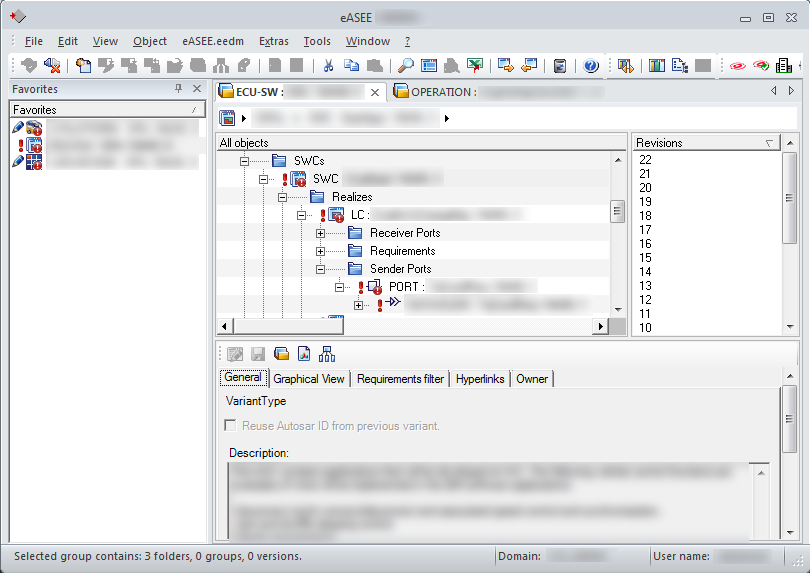
\includegraphics[width=0.95\linewidth]{figure/misc/elektra_screenshot.png}
\caption{A screenshot of the Database}
\label{fig:screenshot_elektra}
\end{figure}

The discussion was for approximately two hours and it was then we figured that we needed to visualize the logical view in the Database which will include LCs, ports and data elements. Håkan also proposed to visualize the physical view in the Database which would include the ECUs. \\

If we describe a bit about what the relationships between ECU and LC are is that, first of all, an ECU can have one to many software compositions (SWCs). The SWC is simply a group of LCs. The LC can have zero to many ports and each port has one data element, it is the data element that connects one LC to another through ports. For example, \texttt{LC 1} with \texttt{PORT 1} can be linked to \texttt{LC 2} with \texttt{PORT 2} only if \texttt{PORT 1} and \texttt{PORT 2} have the same data element.\\

In the discussion with Håkan, we decided to visualize a sub-system. An example of a simple sub-system can be observed from the figure~\ref{fig:hakan-diagram-board} on the top left, there is a small box named SUBSYSTEM and inside of it, there are two ECUs, one ECU has two LCs and another ECU has one LC. The LCs are connected together via ports. The LCs inside the sub-system are also connected to other LCs outside the sub-system but our scope is only for LCs inside a single sub-system. For this report, we will visualize a sub-system named Visibility Control SPA, this sub-system has 18 LCs and 179 ports at the moment.\\


\begin{figure}[H]
\centering
\captionsetup{justification=centering}
\vspace{0cm}% Adjust vertical spacing here
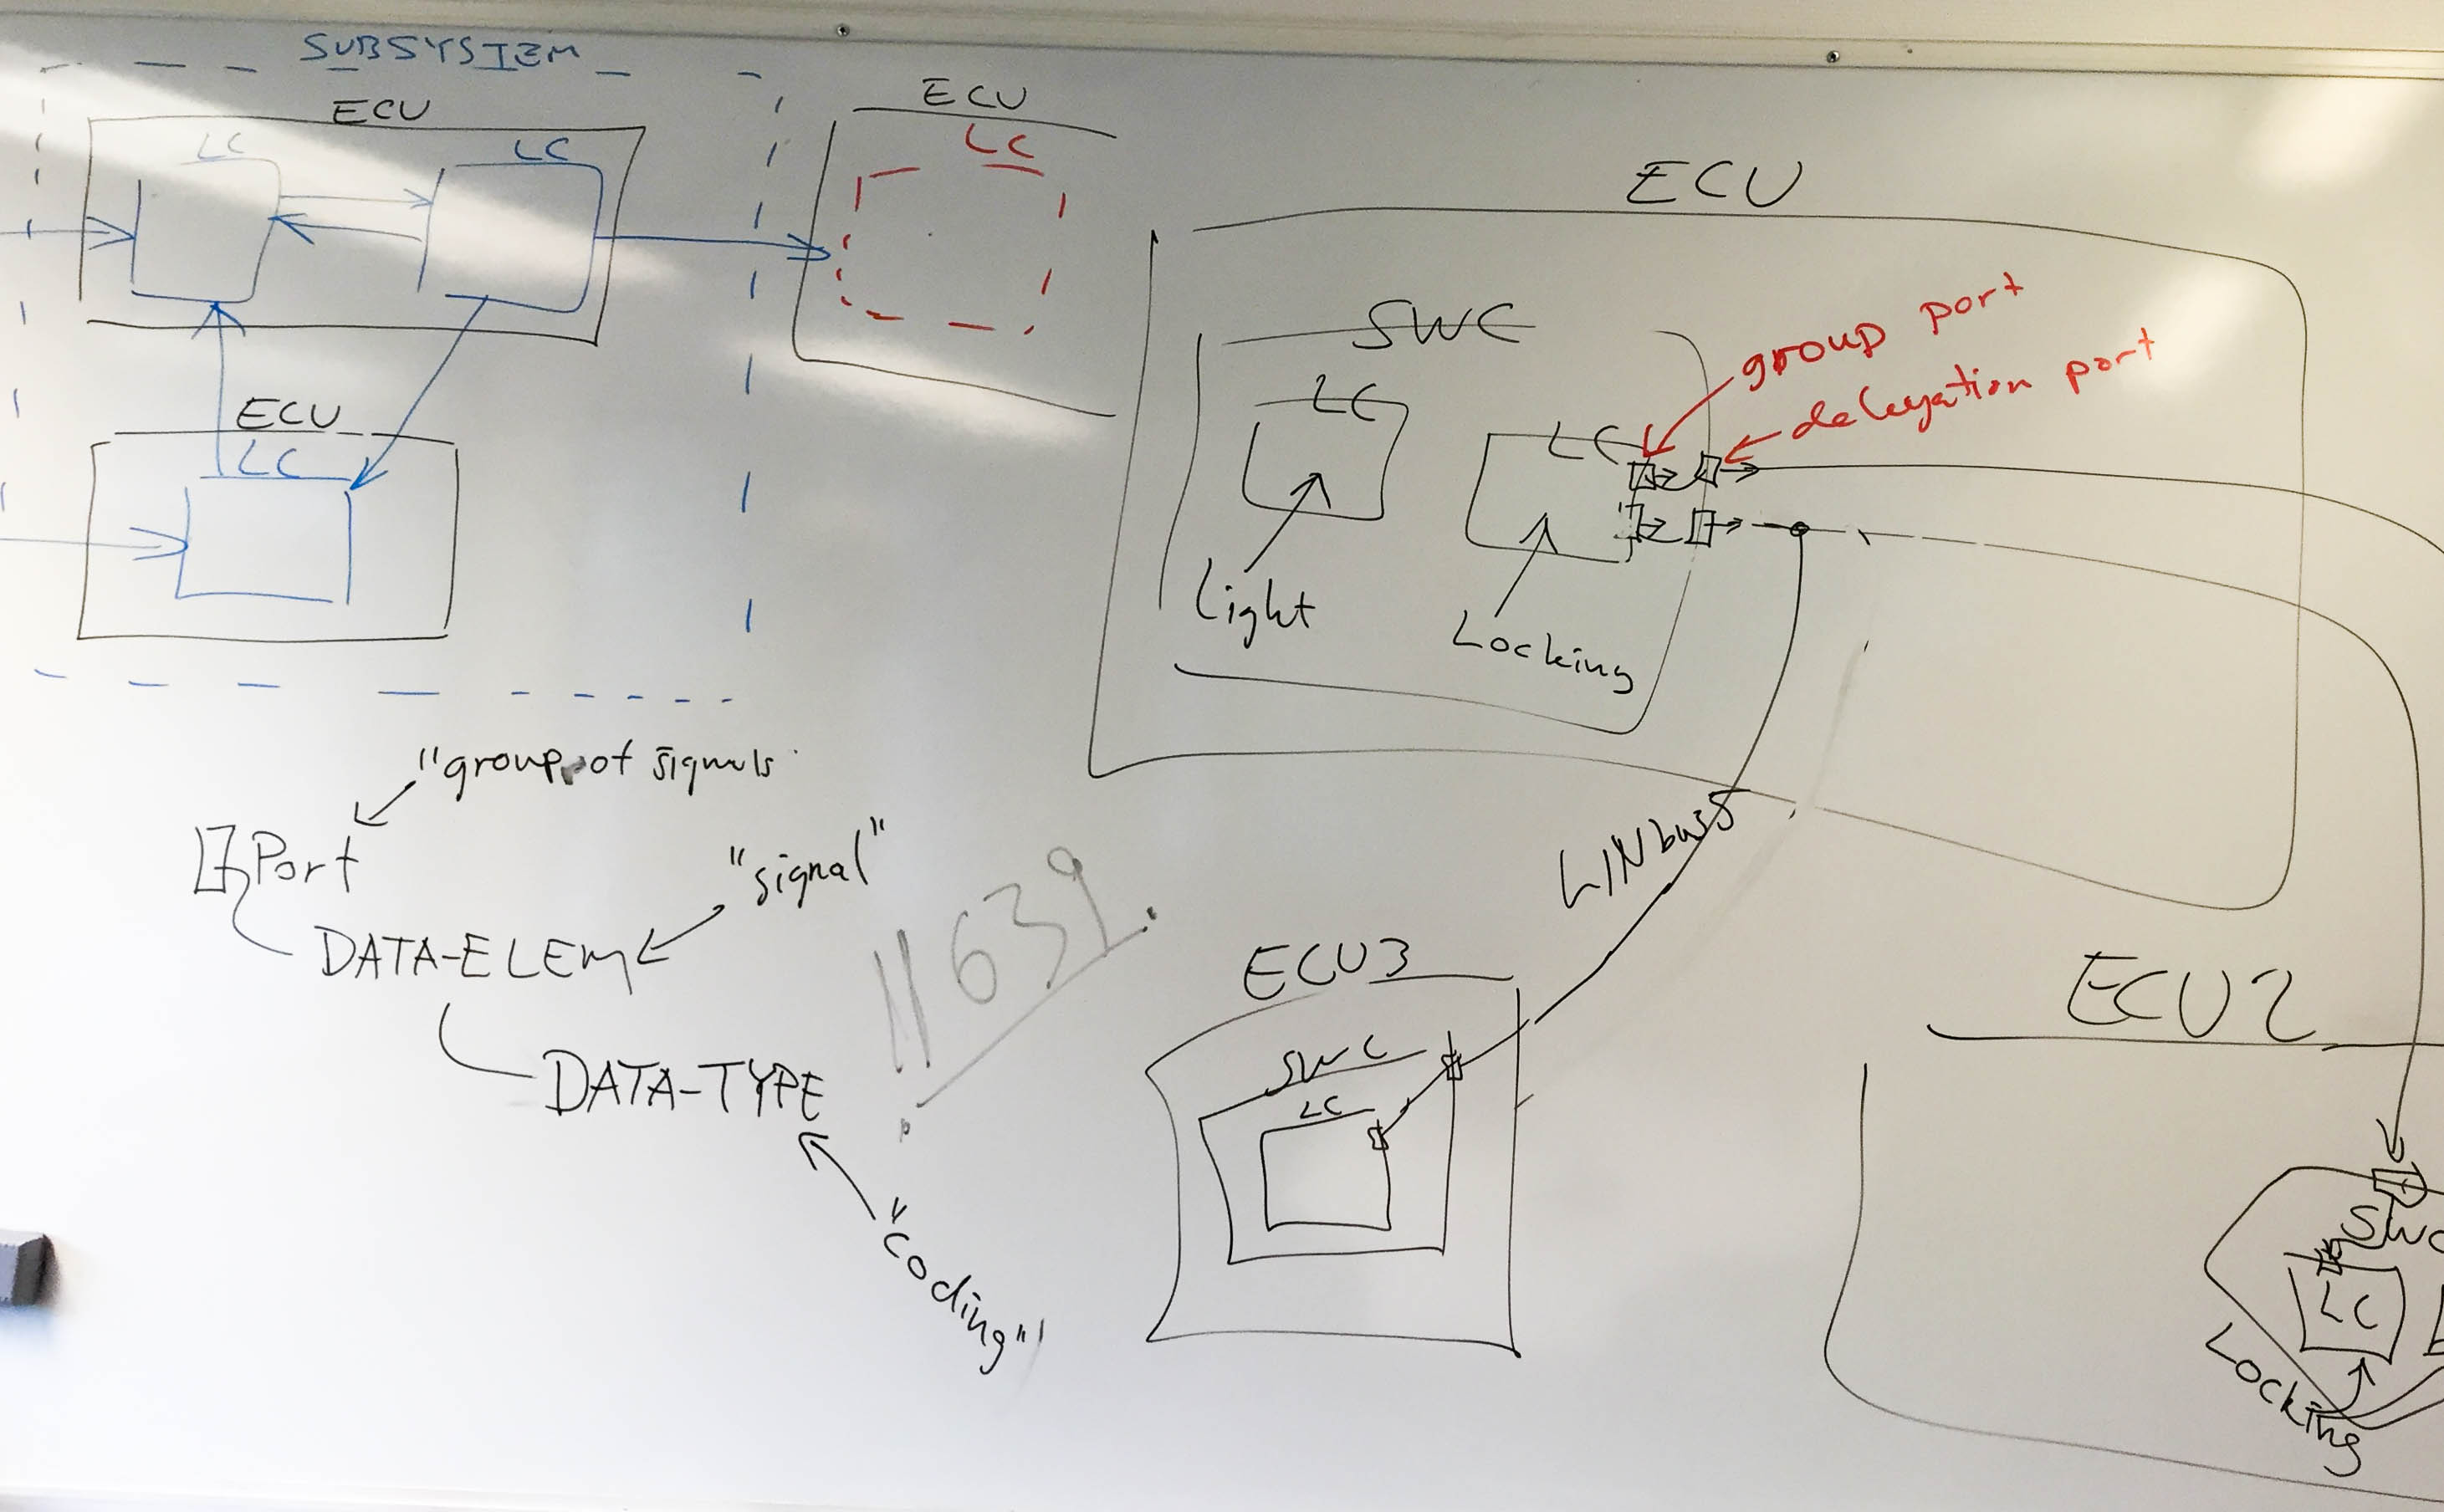
\includegraphics[width=0.85\linewidth]{figure/misc/Hakan.jpg}
\caption{Example of a visualization from a stakeholder}
\label{fig:hakan-diagram-board}
\end{figure}

\subsection{Analyzing the raw JSON data}
\label{IM:analyzing_the_raw_json_data}
On this sub-section, we had to understand the meaning of the JSON objects found on the retrieved data and their relations with one another. The static file had approximately 45 thousands line of code. The beginning of the static file that was retrieved from the Database is shown in the Listing~\ref{code:origin_static_file} below:

\begin{lstlisting}[caption= The section found in the beginning of the visualized static file, label=code:origin_static_file]
{
   "elementName": "Visibility Control SPA", 
    "name": "Visibility Control SPA", 
    "state": "In work", 
    "classType": "GSUBSYSTEM", 
    "variant": "MAIN", 
    "domain": "VCC_EEDM", 
    "creationUser": "Anonymous", 
    "className": "SUBSYSTEM", 
    "contentRelations": [
        {
            "destination": {
                "elementName": "LTC 1", 
                "name": "Name for LTC 1", 
                "classType": "GLTC", 
                "variant": "MAIN", 
                "domain": "VCC_EEDM", 
                "creationUser": "Anonymous", 
                "className": "LTC", 
                "state": "Frozen", 
                "modificationUser": "Anonymous", 
                "modificationDate": "2013-06-25T05:13:36+0000", 
                "attributes": {
                    "MaximumLatency": "250", 
                    "Access control": "Access allowed", 
                    "NominalLatency": "-1", 
                    "RefinedConstraints": [], 
                    .....
                }, 
                "creationDate": "2013-05-02T11:48:25+0000", 
                "id": "1937212", 
                "elementId": "1169278", 
                "revision": 0
            }, 
            "contentAttributes": {}
        }, 
        .....   
}
\end{lstlisting}

From the Listing~\ref{code:origin_static_file} shown above, the variable \texttt{elementName} that appears in Line 1 of the file specifies the name of the sub-system that is visualized which has the value \texttt{Visibility Control SPA}. The variable \texttt{className} that appears in Line 9 determines the class of the static file that is visualized, it has the value \texttt{SUBSYSTEM}. \\

In order to explain the relationships between JSON objects found in the retrieved file, we created a meta-model for the purpose of explaining the contents of the file, see figure~\ref{fig:old_metamodel} below.

\begin{figure}[H]
\centering
\captionsetup{justification=centering}
\vspace{0cm}% Adjust vertical spacing here
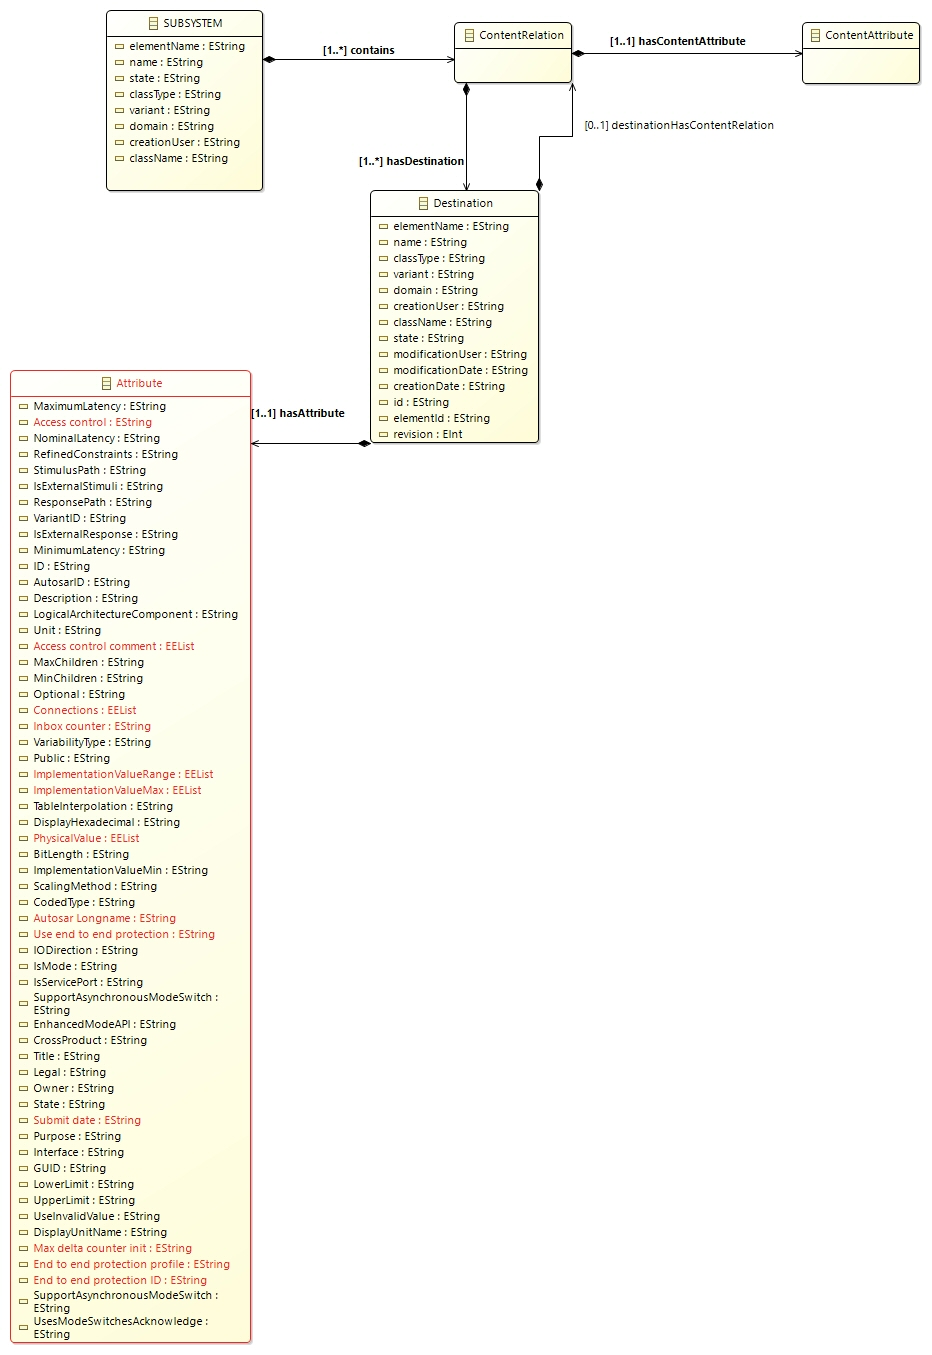
\includegraphics[width=0.45\linewidth]{figure/new_model/Old_Metamodel.jpg}
\caption{A meta-model to explain the content of the retrieved data from the Database}
\label{fig:old_metamodel}
\end{figure}

The meta-model shown in the figure~\ref{fig:old_metamodel} has sum up most of the variables found in the static file. The classes that we needed the most are the \texttt{contentRelations}, \texttt{destination} and \texttt{attributes}. It can be noticed that the class \texttt{contentRelations} has an association of one to many with the class \texttt{destination} and also the class \texttt{destination} has an association of zero to one with the class \texttt{contentRelations}. Also, the class \texttt{destination} has an association of one to one with the class \texttt{attribute}. \\

The objects of the class \texttt{destination} could be LC, port, data-element, data-type, REQSET, etc. In order to elaborate this, we will give an explanation of how it appears in the JSON file : \\

\begin{enumerate}
\item a LC which is a JSON object of a class \texttt{destination} has a JSON object of a class \texttt{contentRelations}, let's name it \texttt{CR1},
\item a JSON object \texttt{CR1} can have an array of JSON objects of a class \texttt{destinations}, a port being one of the JSON object of a class \texttt{destination} in that array,
\item a port has a JSON object of a class \texttt{contentRelations}, let's name it \texttt{CR2},
\item a JSON object \texttt{CR2} can have an array of JSON objects of a class \texttt{destinations}, a data-element being one of the JSON object of a class \texttt{destination} in that array,
\item a data-element has a JSON object of a class \texttt{contentRelations}, let's name it \texttt{CR3},
\item a JSON object \texttt{CR3} can have an array of JSON objects of a class \texttt{destinations}, a data-type being one of the object of a class \texttt{destination}, etc.\\
\end{enumerate} 

The Listing~\ref{code:lc_port_dataElem} below presents the LC 1, its port and its data element, some data have been omitted to allow the possibilities to see how the LC, port, data-element and data-type are related: \\

\begin{lstlisting}[caption={A sample part of a JSON file showing the relationship between LC, port and data-element},label=code:lc_port_dataElem]
{
  "destination": {
      "elementName": "LC 1", 
      "name": "Name for LC 1", 
       ....., 
      "contentRelations": [
            {
            "destination": {
                "elementName": "PORT 1", 
                "name": "Name for PORT 1", 
                  ....., 
                 "contentRelations": [
                      {
                      "destination": {
                           "elementName": "DATA-ELEM 1", 
                           "name": "Name for DATA-ELEM 1", 
                            .... 
                           "contentRelations": [
                                 {
                                  "destination": {
                                  "elementName": "DATA-TYPE 1", 
                                  "name": "Name for DATA-TYPE 1",    .....,   
                "attributes": {
                    "IODirection": "REQUIRE",
                    ...
}\\
\end{lstlisting}

A JSON object with the name \texttt{attributes} can be noticed from the Listing~\ref{code:lc_port_dataElem} at line 145, inside this object, there is a variable with the name \texttt{IODirection}. The variable \texttt{IODirection} determines whether a port provides to another port or a port requires another port. The principle in this context of require and provide is that it explains about a dependency between ports and when it comes to visualize the connection between LCs, we took a look at this variable to determine on how to map the ports in a visualized component diagram.

\subsection{Optimizing the raw JSON data}
The data retrieved from the Database had so many information that were somehow not needed in the visualization. The first step we did was to find a way to omit the data that was not needed and keep the one that we only needed to visualize. The optimized JSON content was applied to the JSON discover to get the metamodel and the model instance. The last part of implementation involved writing a generator with Acceleo template engine and visualized the text generated with PlantUML.\\

As it can be observed in the listing~\ref{code:origin_static_file}, the raw JSON data had lots of information that was necessary to be filtered. What we did was to write an algorithm that is able to read the original JSON data and get only the data that we used in the visualization. The optimized data included the names of LCs, the ports for each LCs, the name of the ports, the \texttt{IODirection} of the port which determines the connection between the ports and the data-element of the ports.\\

To explain how the algorithm works, we will write down the steps that we followed:
\begin{enumerate}
\item Read from a original JSON file
\item Get the name of the sub-system
\item Introduce loop 1 that gets all the LCs of the sub-system.
\item Introduce loop 2 inside loop 1 that gets all the ports of a single LC
\item Get the name of the port
\item Get the name of the data-element
\item Get the value of \texttt{IODirection} of the port
\item End of the loop 2, End of loop 1
\item Write an optimized content to a new file
\end{enumerate}

The result of the algorithm that does a JSON optimization appears in the listing\ref{code:optimized_JSON} below :

\begin{lstlisting}[caption=A sample part of the optimized JSON content,label=code:optimized_JSON]
{
  "elementName": "Visibility Control SPA",
  "hasLC": [
    {
      "elementName": "LC 1",
      "hasPort": [
        {
          "elementName": "PORT 1",
          "IOdirection": "REQUIRE",
          "dataElement": "DATA-ELEM 1"
        }
      ]
    },
    {
      "elementName": "LC 2",
      "hasPort": []
    },
    {
      "elementName": "LC 3",
      "hasPort": [
        {
          "elementName": "PORT 2",
          "IOdirection": "REQUIRE",
          "dataElement": "DATA-ELEM 2"
        },
        {
          "elementName": "PORT 3",
          "IOdirection": "REQUIRE",
          "dataElement": "DATA-ELEM 3"
        }
        ....
}
\end{lstlisting}


\subsection{Creating a new meta-model and model instance}
Once the raw JSON data is optimized (Listing~\ref{code:optimized_JSON}), we created a meta-model and a model instance using the open-source tool JSON discoverer. Before getting to the point where we obtained the meta-model and the model instance, we want to explain how process the discovering of JSON schema works. Based on the paper written by the tool creators Javier Luis Cánovas Izquierdo and Jordi Cabot~\cite{Canovas}, the discovering process is a model-based process which is composed of three phases:  pre-discovery phase, single-service discovery phase, and multi-service discovery
phase. The first phase aims to extract the low-level a JSON model out of a JSON document. The second phase is to obtain the schema information of a JSON document. The last phase aims at obtaining common schema of more than one JSON documents. Since the data of the sub-system Visiblity Control SPA that we extracted from the Database was in one single JSON document, multi-service discovery phase was not part of the work. \\

With the optimized version of the raw JSON file, JSON discover provided us a very-simple-but-efficient meta-model. From Figure~\ref{fig:new_metamodel}, the meta-model comprises three classes \texttt{SubSystem}, \texttt{HasLC}, and \texttt{HasPort}. Each class has at least one attribute (property). \texttt{SubSystem} has an attribute \texttt{elementName} which represents the name of sub-system. The class \texttt{HasLC} has one attribute \texttt{elementName} which represents the name of LC. The class \texttt{HasPort} has three attributes namely \texttt{elementName} containing the name of port, \texttt{IODirection} specifying the type of port (\texttt{PROVIDE} or \texttt{REQUIRE}), and \texttt{dataElement} keeping the name of port. All attributes are of type \texttt{String}.

\begin{figure}[H]
\centering
\captionsetup{justification=centering}
\vspace{0cm}% Adjust vertical spacing here
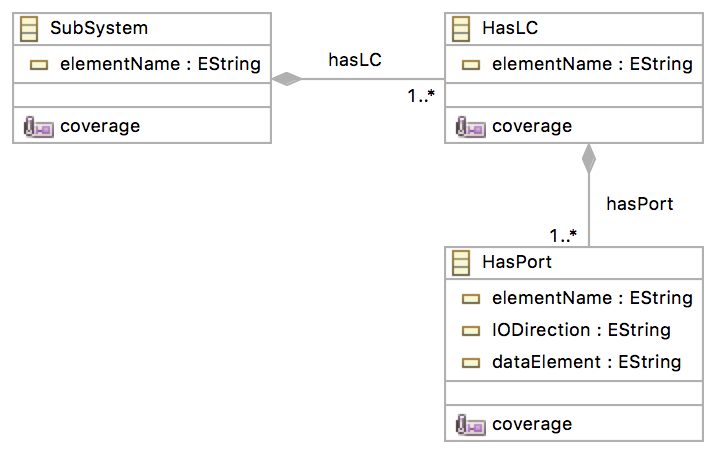
\includegraphics[width=0.65\linewidth]{figure/new_model/new_metamodel.png}
\caption{The meta-model of the optimized JSON document discovered by JSON discoverer tool}
\label{fig:new_metamodel}
\end{figure}

The meta-model also has two class relationships: \texttt{hasLC} and \texttt{hasPort}. The first relationship is a composition meaning that the class \texttt{HasLC} will be destroyed if the class \texttt{SubSystem} is destroyed. The same type of relationship is also applied to the relationship between the class \texttt{HasLC} and \texttt{HasPort}. Both relationships have multiplicity \texttt{1..*} according to the optimized JSON document. Note that the annotations \texttt{coverage} included in all classes are resulted from the the JSON grammar rules the authors of JSON discoverer created to guide the generation of the JSON meta-model~\cite{Canovas}. \\

As it has been mentioned that JSON discoverer also provides the discovery of data model (model instance). Using the same optimized JSON document, we obtained a model instance in XML\footnote{Extensible Markup Language} Metadata Interchange (XMI) file. A part of the file can be seen in Listing~\ref{code:model_instance_xmi}.

\begin{lstlisting}[caption=Data model or model instance discovered by JSON discoverer,label=code:model_instance_xmi]
<?xml version="1.0" encoding="UTF-8"?>
<discoD:SubSystem
    xmi:version="2.0"
    xmlns:xmi="http://www.omg.org/XMI"
    xmlns:xsi="http://www.w3.org/2001/XMLSchema-instance"
    xmlns:discoD="http://jsonDiscoverer/discovered/SubSystem"
    xsi:schemaLocation="http://jsonDiscoverer/discovered/SubSystem metamodel.ecore" elementName="Visibility Control SPA">
  <hasLC elementName="LC 1">
    <hasPort elementName="PORT 1" IODirection="REQUIRE" dataElement="DATA-ELEM 1"/>
  </hasLC>
  ...
</discoD:SubSystem>
\end{lstlisting}

Using the editor from the EcoreTools Eclipse plug-in, the model instance and the properties of each class are visualized as seen in Figure~\ref{fig:new_model_instance}. From the model instance (left), it can be seen that the attribute \texttt{elementName} of the class \texttt{SubSystem} is \texttt{"Visibility Control SPA"}. It has 18 children (\texttt{HasLC}), \texttt{LC 1}, \texttt{LC 2}, \texttt{LC 3}, ..., \texttt{LC 18}. Each child has its own \texttt{HasPort}, \texttt{PORT 1} belongs to \texttt{LC 1}, for example. The properties of each class are shown on the right side of the figure. Note that the model instance was constructed conforming to the meta-model in Figure~\ref{fig:new_metamodel}.

\begin{figure}[H]
\centering
\captionsetup{justification=centering}
\vspace{0cm}% Adjust vertical spacing here
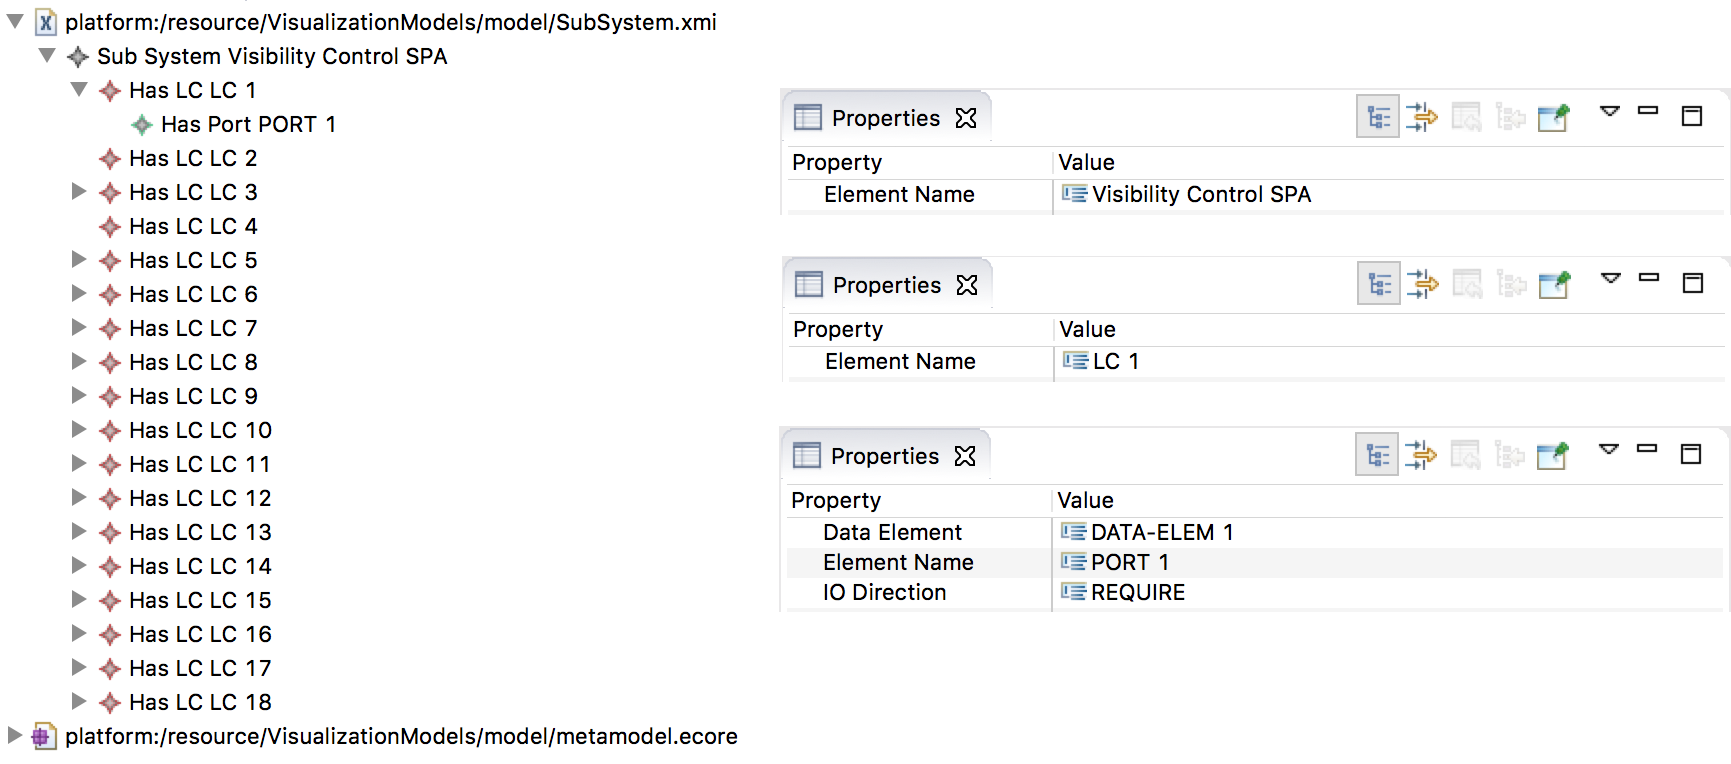
\includegraphics[width=0.95\linewidth]{figure/new_model/new_model_instance.png}
\caption{The model instance resulted from the optimized JSON document}
\label{fig:new_model_instance}
\end{figure}

\subsection{Automated visualization prototype}
\label{IM:automated_visualization_prototype}
Up to this point, we already had the meta-model and the model-instance from the optimized JSON document. The next step was to do M2T transformation, which could be done by create an Acceleo template for textual description. The complete template is included in Appendix~\ref{app1} Section~\ref{app1:prototype}. Only important pieces of code will be explained in this section.\\

\subsubsection*{Defining sub-system}
\begin{lstlisting}[caption=Defining \texttt{artifact} for the sub-system,label=code:defining_subsystem]
...
[template public generateElement(subsystem : SubSystem)]
...
artifact [subsystem.elementName.replaceAll(' ', '')/] {
...
}
\end{lstlisting}

The sub-system \texttt{Visibility Control SPA} is visualized as an \texttt{artifact} following by its name. To be able to get the name, we first created a \texttt{SubSystem}-type parameter, namely \texttt{subsystem}. With this parameter, we could access its attribute \texttt{elementName}. A \texttt{replace} operation is used to remove white space in the value because PlantUML does not support name with white space. Thus, the name printed in the visualization is \texttt{VisibilityControlSPA}.

\subsection*{Defining LCs}

\begin{lstlisting}[caption=Defining \texttt{component} for the LCs,label=code:defining_lc]
...
[for (lc:HasLC | subsystem.hasLC)]
['['/][lc.elementName.replace(' ', '')/][']'/]
[/for]
...
\end{lstlisting}

Inside the \texttt{artifact}, a for-loop statement is implemented for retrieving all LCs belonging to the sub-system. The for-loop has a parameter \texttt{lc} belonging to the class \texttt{HasLC} which can be accessed via the class relationship \texttt{hasLC}. The name of the LCs can be obtained by \texttt{lc.elementName}, and the \texttt{replace} operation is used as well to remove white space.


\subsection*{Defining ports and connections}

\begin{lstlisting}[caption=Defining ports and connections,label=code:defining_ports_connections]
...
[for (lc:HasLC | subsystem.hasLC)]
[for (port:HasPort | lc.hasPort)]
[for (lc2:HasLC | subsystem.hasLC)]
[for (port2:HasPort | lc2.hasPort)]
[if ((port2.dataElement = port.dataElement) and not (port2.elementName = port.elementName) and not (lc.elementName = lc2.elementName)) and (lc2.elementName.replace(' ', '').substring(3).toInteger() > lc.elementName.replace(' ', '').substring(3).toInteger())]
[if not (port.IODirection = port2.IODirection)]
[lc.elementName.replace(' ', '')/] "[port.elementName.substring(6)/]['-'/][port.dataElement.substring(11)/]" [if (port.IODirection = 'REQUIRE')]#--([elseif (port.IODirection = 'PROVIDE')]#--0[/if][if (port2.IODirection = 'REQUIRE')])--#[elseif (port2.IODirection = 'PROVIDE')]0--#[/if] "[port2.elementName.substring(6)/]['-'/][port2.dataElement.substring(11)/]" [lc2.elementName.replace(' ', '')/]
[elseif (port.IODirection = port2.IODirection)]
[/if]
[/if]
[/for]
[/for]
[/for]
[/for]
...
\end{lstlisting}

Ports and connections in textual description has to be in the same line, in the following syntax:\\
\begin{center}
\texttt{$A_1$ "$B_1$-$C_1$" \#--(0--\# "$B_2$-$C_2$" $A_2$}
\end{center}
\vspace{1em}
Assume that \texttt{A} is the name of a LC, \texttt{B} is the number part of a port name, for example, \texttt{1} is the number part of \texttt{PORT 1}, and \texttt{C} is the number part of data element of the port. The connection between two ports was defined based on the type of a port (attribute \texttt{IODirection}), \texttt{\#--(} for REQUIRE port and \texttt{\#--O} for PROVIDE port. \\

To obtain the name of all LCs and their ports, we created a new for-loop looping through \texttt{HasLC} and an inner for-loop to get port(s) of each LC looping through \texttt{HasPort}. This results in obtaining \texttt{$A_1$ "$B_1$-$C_1$"}. After that, we created another two for-loops inside the inner for-loop in order to search for each LC's pair, resulting in obtaining \texttt{"$B_2$-$C_2$" $A_2$}. An if-statement is used to pair two ports by checking if their attributes \texttt{dataElement} have the same value, and validate that the two LCs are not the same LC. For the connection between two ports, two if-statements are created, one to check the type of each port, and another to pair between two ports having different types. This results in having two representations of connections as follow:
\vspace{0.5em}
\begin{itemize}
    \item REQUIRE-PROVIDE, \texttt{\#--(0--\#}
    \item PROVIDE-REQUIRE, \texttt{\#--0)--\#}
\end{itemize}
\vspace{1em}
From the template, Acceleo generated a textual description that could be visualized using PlantUML. Listing~\ref{code:plantuml_textual} shows a piece of it.

\begin{lstlisting}[caption=A piece of textual representation generated from Acceleo template engine,label=code:plantuml_textual]
@startuml

skinparam nodesep 80
skinparam ranksep 80

artifact VisibilityControlSPA {
[LC1]
[LC2]
[LC3]
...
LC1 "1-1" #--(0--# "165-1" LC18
LC3 "2-2" #--(0--# "144-2" LC17
LC3 "4-4" #--(0--# "116-4" LC10
...
}

@enduml
\end{lstlisting}

The result from the textual description is presented in Chapter~\ref{results} Section~\ref{RE:automated_visualization_prototype}.

The automated visualization prototype of the sub-system \texttt{Visibility Control SPA} can be seen in Section~\ref{RE:automated_visualization_prototype}.

\subsection{Final version of the automated visualization}
Once the automated visualization prototype was created, we arranged the second meeting with Håkan for presenting the prototype and getting some feedback regarding the prototype. We found out that the most important information that should be included in the visualization was the \texttt{dataElement} properties of the class \texttt{HasPort}, not \texttt{elementName}. Because of this reason, we improved the automated visualization by introducing a representation for data element as well as redefining sub-system, and ports and connections.

\subsection*{Defining data element}
\begin{lstlisting}[caption=Defining \texttt{rectangle} for the data element,label=code:defining_dataelements]
...
[for (lc:HasLC | subsystem.hasLC)]
[for (port:HasPort | lc.hasPort)]
rectangle [port.dataElement.replace('-','').replace(' ','')/]
[/for]
[/for]
...
\end{lstlisting}

\texttt{Rectangle} was used for representing all data elements provided/required by ports. Two for-loop statements was created. The first one is for retrieving all LCs belonging to the sub-system. The second one is for retrieving all ports belonging to each LC. The data element can be obtained by \texttt{port.dataElement}, and two replace operations are used as well to remove dash symbol and white space.

\subsection*{Redefining sub-system}
\begin{lstlisting}[caption=Redefining \texttt{package} for the sub-system,label=code:redefining_subsystem]
...
package "[subsystem.elementName.replaceAll(' ', '')/]"{
...
}
...
\end{lstlisting}

Sub-system was redefined from Section~\ref{IM:automated_visualization_prototype}. Instead of using \texttt{artifact}, \texttt{rectangle} is used to represent the sub-system.

\subsection*{Redefining ports and connections}
\begin{lstlisting}[caption=Redefining ports and connection,label=code:redefining_ports_and_connection]
...
[for (lc:HasLC | subsystem.hasLC)]
[for (port:HasPort | lc.hasPort)] 
[if (port.IODirection = 'PROVIDE')] 
['['/][lc.elementName.replace(' ', '')/][']'/] -0 [port.dataElement.replace('-','').replace(' ','')/]
[/if]
[if (port.IODirection = 'REQUIRE')]
['['/][lc.elementName.replace(' ', '')/][']'/] -( [port.dataElement.replace('-','').replace(' ','')/]   
[/if]
[/for]
[/for]
...
\end{lstlisting}

Ports and connection syntax was redefined as follow:\\
\begin{center}
\texttt{$A$ -( $D$}
\end{center}
\vspace{1em}
Assume that \texttt{A} is the name of a LC, and \texttt{D} is the data element. The connection between a port and its data element was defined based on the type of a port (attribute \texttt{IODirection}), \texttt{-(} for \texttt{REQUIRE} port and \texttt{-O} for \texttt{PROVIDE} port. \\

From the template, Acceleo generated a textual description for the final version of the automated visualization. Listing~\ref{code:plantuml_textual_final} shows a piece of it.

\begin{lstlisting}[caption=A piece of textual representation generated from Acceleo template engine for the final version of the automated visualization,label=code:plantuml_textual_final]
@startuml
...
package "VisibilityControlSPA"{
rectangle DATAELEM1
rectangle DATAELEM2
rectangle DATAELEM3
...
[LC1] -up-( DATAELEM1     
[LC3] -up-( DATAELEM2     
[LC3] -up-( DATAELEM3
...
}
@enduml
\end{lstlisting}

The result from the textual description is presented in Chapter~\ref{results} Section~\ref{RE:final_version_of_the_automated_visualization}.

%------------------------------------------------------------------%
%%%%%%
\section{Identifying the needs of stakeholders}
 
\subsection{Selecting a group of stakeholders}
\todo{should be fixed}
Since the visualization is based on a single sub-system \texttt{Visibility Control SPA}, we would prefer to interview the stakeholders that uses this sub-system often. These were the primary stakeholders since they are directly interacting with the the Database.


\subsection{Preparation for the interviews}
\todo{should be fixed}
Basili~\cite{Basili} has explained couple of steps to follow when collecting data. We have applied the first two steps mentioned in his work, the steps are establishing the goals for data collection and developing a list of questions of interests. The goals we set for this interview were getting to know important artifacts on the visualization from the each stakeholder, getting to know the artifacts that most stakeholder needs in their line of work, finding the metrics that we could use to determine the important artifacts and also understanding the needs of the stakeholders.

\subsection{Coding the interview transcripts}
\label{IM:coding_the_interview_transcripts}
\todo{how we code}

\subsection{Categorizing the needs of stakeholders}
\todo{how we categorize the needs}
